\documentclass[12pt]{report}
\usepackage[utf8]{inputenc}
\usepackage[russian]{babel}
%\usepackage[14pt]{extsizes}
\usepackage{listings}
\usepackage{graphicx}
\usepackage{amsmath,amsfonts,amssymb,amsthm,mathtools} 
\usepackage{pgfplots}
\usepackage{filecontents}
\usepackage{float}
\usepackage{comment}
\usepackage{indentfirst}
\usepackage{eucal}
\usepackage{enumitem}
%s\documentclass[openany]{book}
\frenchspacing

\usepackage{indentfirst} % Красная строка

\usetikzlibrary{datavisualization}
\usetikzlibrary{datavisualization.formats.functions}

\usepackage{amsmath}


% Для листинга кода:
\lstset{ %
	language=c,                 % выбор языка для подсветки (здесь это С)
	basicstyle=\small\sffamily, % размер и начертание шрифта для подсветки кода
	numbers=left,               % где поставить нумерацию строк (слева\справа)
	numberstyle=\tiny,           % размер шрифта для номеров строк
	stepnumber=1,                   % размер шага между двумя номерами строк
	numbersep=5pt,                % как далеко отстоят номера строк от подсвечиваемого кода
	showspaces=false,            % показывать или нет пробелы специальными отступами
	showstringspaces=false,      % показывать или нет пробелы в строках
	showtabs=false,             % показывать или нет табуляцию в строках
	frame=single,              % рисовать рамку вокруг кода
	tabsize=2,                 % размер табуляции по умолчанию равен 2 пробелам
	captionpos=t,              % позиция заголовка вверху [t] или внизу [b] 
	breaklines=true,           % автоматически переносить строки (да\нет)
	breakatwhitespace=false, % переносить строки только если есть пробел
	escapeinside={\#*}{*)}   % если нужно добавить комментарии в коде
}


\usepackage[left=2cm,right=2cm, top=2cm,bottom=2cm,bindingoffset=0cm]{geometry}
% Для измененных титулов глав:
\usepackage{titlesec, blindtext, color} % подключаем нужные пакеты
\definecolor{gray75}{gray}{0.75} % определяем цвет
\newcommand{\hsp}{\hspace{20pt}} % длина линии в 20pt
% titleformat определяет стиль
\titleformat{\chapter}[hang]{\Huge\bfseries}{\thechapter\hsp\textcolor{gray75}{|}\hsp}{0pt}{\Huge\bfseries}


% plot
\usepackage{pgfplots}
\usepackage{filecontents}
\usetikzlibrary{datavisualization}
\usetikzlibrary{datavisualization.formats.functions}

\begin{document}
	%\def\chaptername{} % убирает "Глава"
	\thispagestyle{empty}
	\begin{titlepage}
		\noindent \begin{minipage}{0.15\textwidth}
			
\includegraphics[width=\linewidth]{img/b_logo}
		\end{minipage}
		\noindent\begin{minipage}{0.9\textwidth}\centering
			\textbf{Министерство науки и высшего образования Российской Федерации}\\
			\textbf{Федеральное государственное бюджетное образовательное учреждение высшего образования}\\
			\textbf{~~~«Московский государственный технический университет имени Н.Э.~Баумана}\\
			\textbf{(национальный исследовательский университет)»}\\
			\textbf{(МГТУ им. Н.Э.~Баумана)}
		\end{minipage}
		
		\noindent\rule{18cm}{3pt}
		\newline\newline
		\noindent ФАКУЛЬТЕТ $\underline{\text{«Информатика и системы управления»}}$ \newline\newline
		\noindent КАФЕДРА $\underline{\text{«Программное обеспечение ЭВМ и информационные технологии»}}$\newline\newline\newline\newline\newline
		
		\begin{center}
			\noindent\begin{minipage}{1.1\textwidth}\centering
				\Large\textbf{  Отчет по лабораторной работе №5}\newline
				\textbf{по дисциплине <<Компьютерные сети>>}\newline\newline\newline
			\end{minipage}
		\end{center}
		
		\noindent\textbf{Тема} $\underline{\text{Протокол SMTP. Реализация SMTP-клиента}}$\newline\newline
		\noindent\textbf{Студент} $\underline{\text{Романов А.В.~~~~~~~~~~~}}$\newline\newline
		\noindent\textbf{Группа} $\underline{\text{ИУ7-73Б~~~~~~~~~~~~~~~~~~~}}$\newline\newline
		\noindent\textbf{Преподаватель} $\underline{\text{Рогозин Н. О.}}$\newline\newline\newline
		
		\begin{center}
			\vfill
			Москва~---~\the\year
			~г.
		\end{center}
	\end{titlepage}


\section*{Задание}

Написать SMTP-клиент, который:

\begin{itemize}
	\item в качестве вводных данных (аргументы командной строки) получает: адрес получателя, адрес отправителя, пароль;
	\item использует один из открытых SMTP-серверов для доставки MIME-сообщений, включая приложения, если они есть, в соответствии с вариантом;
\end{itemize}

\textbf{Вариант №12, дополнительное задание №1.} Доставка сообщений выполняется с регулярным интервалом. Интервал и тело сообщения, имя файла для прикрепления (опционально) вводятся с клавиатуры.

\section*{Код программы}


\begin{lstlisting}[label=lst:lab_04,caption=Реализация SMTP-клиента,language=python]
import argparse
import os
import smtplib
import sys
from email.mime.application import MIMEApplication
from email.mime.multipart import MIMEMultipart
from email.mime.text import MIMEText
from os.path import basename
from time import sleep


def get_args():
	parser = argparse.ArgumentParser()
	parser.add_argument('mail_to', action="store", help="Email address: to")
	parser.add_argument('mail_from', action="store", help="Email address: from")
	parser.add_argument('password_from', action="store", help="Password: from")
	parser.add_argument('-a', '--attachment', action="store", required=False, help="Attach file")
	return parser


def add_file(msg, fname):
	with open(fname, "rb") as fl:
		part = MIMEApplication(fl.read(), Name=basename(fname))
		part['Content-Disposition'] = 'attachment; filename="%s"' % basename(fname)
		msg.attach(part)

	return msg


def send_mail(msg, msg_text, smtphost, mail_from, password_from, mail_to, interval, attachment):
	msg['From'] = mail_from
	msg['To'] = mail_to
	msg['Subject'] = "BMSTU CN COURSE LW05"
	msg.attach(MIMEText(msg_text, 'plain'))
	
	if attachment is not None:
		msg = add_file(msg, attachment)
	
	server = smtplib.SMTP(smtphost[0], smtphost[1])
	server.starttls()
	server.login(mail_from, password_from)
	
	while True:
		server.sendmail(msg['From'], msg['To'], msg.as_string())
		print("Email sent from %s to %s" % (msg['From'], msg['To']))
		sleep(interval)


def main():
	parser = get_args()
	
	try:
		args = parser.parse_args(sys.argv[1:])
	except:
		sys.exit("Error in sending email: arguments are not valid")
	
	message = MIMEMultipart()
	message_text = input("Please, enter e-mail message: ")
	interval = int(input("Please, enter interval in seconds: "))
	smtphost = ["smtp.mail.ru", 25]
	
	send_mail(message, message_text, smtphost, args.mail_from, args.password_from, args.mail_to, interval, args.attachment)


if __name__ == '__main__':
	main()
\end{lstlisting}

\section*{Результаты работы программы}

На рис. 1 - 5 представлены результаты работы разработанного программного обеспечения.

\begin{figure}[H]
	\begin{center}
		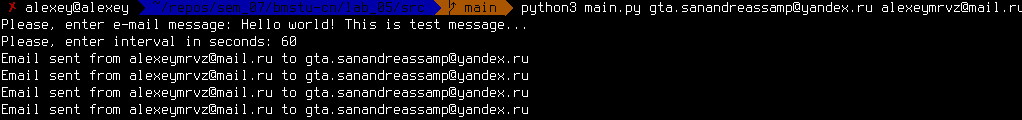
\includegraphics[scale=0.53]{img/1.png}
	\end{center}
	\caption{Запуск клиента без возможности добавить вложение}
	\label{fig:example-no-attachment}
\end{figure}

\begin{figure}[H]
	\begin{center}
		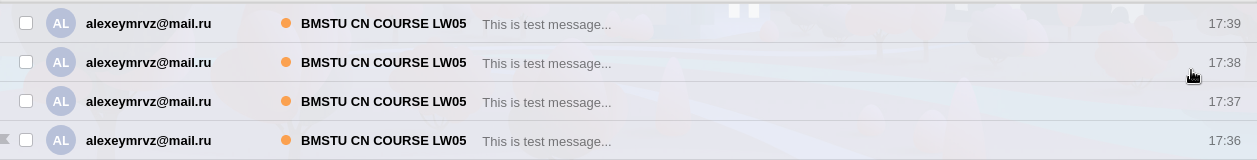
\includegraphics[scale=0.43]{img/2.png}
	\end{center}
	\caption{Сообщения приходят с интервалом 60 секунд}
	\label{fig:example-no-attachment-mail-1}
\end{figure}

\begin{figure}[H]
	\begin{center}
		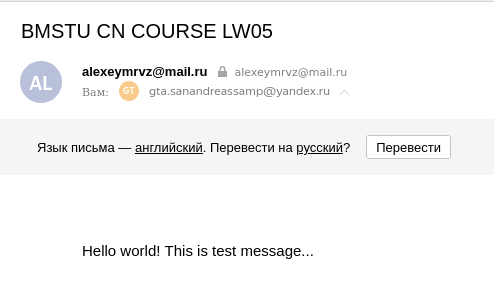
\includegraphics[scale=0.65]{img/3.png}
	\end{center}
	\caption{Содержание письма}
	\label{fig:example-no-attachment-mail-2}
\end{figure}

\begin{figure}[H]
	\begin{center}
		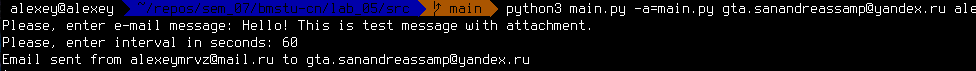
\includegraphics[scale=0.53]{img/4.png}
	\end{center}
	\caption{Запуск клиента с возможностью добавить вложение}
	\label{fig:example-attachment-mail}
\end{figure}

\begin{figure}[H]
	\begin{center}
		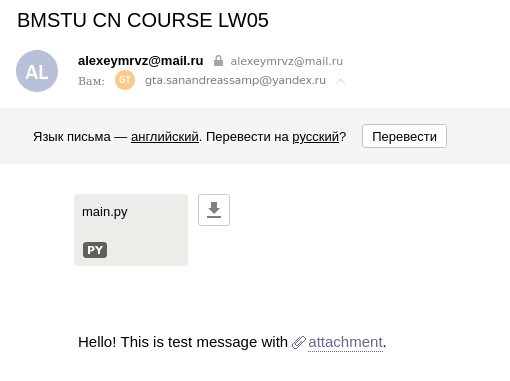
\includegraphics[scale=0.6]{img/5.png}
	\end{center}
	\caption{Содержание письма вместе с вложением}
	\label{fig:example-no-attachment-mail}
\end{figure}

\bibliographystyle{utf8gost705u}
\bibliography{51-biblio}
	
\end{document}
